
\begin{frame}{Przykład konstrukcji}

\begin{columns}
\column{0.35\textwidth}
    \begin{figure}[H]
        \centering
        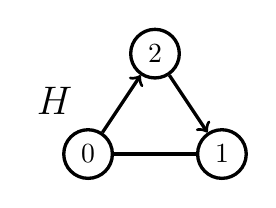
\begin{tikzpicture}[
    scale=0.85,
    minimum size=0.05cm,
    line width=1.2pt
]

    % ----------- Graf H ------------
    \node at (-1.5,1.8) {\Large \(H\)};

    \node[circle, draw=black] (v0) at (-1,1) {\(0\)};
    \node[circle, draw=black] (v1) at (1,1) {\(1\)};
    \node[circle, draw=black] (v2) at (0,2.5) {\(2\)};

    \draw      (v0) -- (v1);
    \draw[->]  (v0) -- (v2);
    \draw[->]  (v2) -- (v1);

\end{tikzpicture}

    \end{figure}
    \uncover<5>{
    \begin{figure}[H]
        \centering
        \begin{tikzpicture}[
    scale=0.85,
    minimum size=0.05cm,
    line width=1.2pt
]

\begin{scope}[shift=({0,-3})]
    \node at (-1.5,1.8) {\Large \(R\)};

    \node[circle, draw=black] (v0) at (-1,1) {\(0\)};
    \node[circle, draw=black] (v1) at (1,1) {\(1\)};
    \node[circle, draw=black] (v2) at (0,2.5) {\(2\)};

    \draw[cfred] (v0) -- (v1);
    \draw[cfred] (v0) -- (v2);
    \draw[cfred, loop left] (v0) to node[left] {} (v0);
    \draw[cfred, loop right] (v1) to node[left] {} (v1);
    \draw[cfred, loop above] (v2) to node[left] {} (v2);
\end{scope}

\end{tikzpicture}

    \end{figure}
    }

\pause
\column{0.65\textwidth}
    \begin{figure}[H]
        \centering
        \begin{tikzpicture}[
    scale=0.8,
    line width=1.2pt,
    minimum size=0.02cm
]

\uncover<2->{
    \node[circle, draw=black] (x0) at (0,0) {};
    \node[circle, draw=black] (x1) at (0.5,0.75) {};
    \node[circle, draw=black] (x2) at (1,1.5) {};
    \node[circle, draw=black] (x3) at (1.5,0.75) {};
    \node[circle, draw=black] (x4) at (2,0) {};

    \draw[->] (x0) -- (x1);
    \draw[->] (x1) -- (x2);
    \draw[->] (x3) -- (x2);
    \draw[->] (x4) -- (x3);
}
\uncover<2>{
    \node[circle, draw=black] (x5) at (2.5,0.75) {};
    \node[circle, draw=black] (x6) at (3,1.5) {};
    \node[circle, draw=black] (x7) at (3.5,0.75) {};
    \node[circle, draw=black] (x8) at (4,0) {};

    \draw[->] (x4) -- (x5);
    \draw[->] (x5) -- (x6);
    \draw[->] (x7) -- (x6);
    \draw[->] (x8) -- (x7);
}

\uncover<3->{
    \node[circle, draw=cfgrey] (x5) at (2.5,0.75) {};
    \node[circle, draw=cfgrey] (x6) at (3,1.5) {};
    \node[circle, draw=cfgrey] (x7) at (3.5,0.75) {};
    \node[circle, draw=cfgrey] (x8) at (4,0) {};

    \draw[->, cfgrey] (x4) -- (x5);
    \draw[->, cfgrey] (x5) -- (x6);
    \draw[->, cfgrey] (x7) -- (x6);
    \draw[->, cfgrey] (x8) -- (x7);
}
 
\uncover<4->{
    \begin{scope}[shift={(-2,-3)}]
        \node[circle, draw=black, label=below:{\(0\)}] (x0) at (0,0) {};
        \node[circle, draw=black, label=left:{\(2\)}] (x1) at (0.5,0.75) {};
        \node[circle, draw=black, label=above:{\(1\)}] (x2) at (1,1.5) {};
        \node[circle, draw=black, label=right:{\(2\)}] (x3) at (1.5,0.75) {};
        \node[circle, draw=black, label=below:{\(0\)}] (x4) at (2,0) {};

        \draw[->] (x0) -- (x1);
        \draw[->] (x1) -- (x2);
        \draw[->] (x3) -- (x2);
        \draw[->] (x4) -- (x3);
    \end{scope}
    \begin{scope}[shift={(1.25,-3)}]
        \node[circle, draw=black, label=below:{\(0\)}] (x0) at (0,0) {};
        \node[circle, draw=black, label=left: {\(2\)}] (x1) at (0.5,0.75) {};
        \node[circle, draw=black, label=above:{\(1\)}] (x2) at (1,1.5) {};
        \node[circle, draw=black, label=right:{\(0\)}] (x3) at (1.5,0.75) {};
        \node[circle, draw=black, label=below:{\(1\)}] (x4) at (2,0) {};

        \draw[->] (x0) -- (x1);
        \draw[->] (x1) -- (x2);
        \draw[->] (x3) -- (x2);
        \draw[->] (x4) -- (x3);
    \end{scope}
    \begin{scope}[shift={(4.5,-3)}]
        \node[circle, draw=black, label=below:{\(0\)}] (x0) at (0,0) {};
        \node[circle, draw=black, label=left: {\(1\)}] (x1) at (0.5,0.75) {};
        \node[circle, draw=black, label=above:{\(0\)}] (x2) at (1,1.5) {};
        \node[circle, draw=black, label=right:{\(1\)}] (x3) at (1.5,0.75) {};
        \node[circle, draw=black, label=below:{\(2\)}] (x4) at (2,0) {};

        \draw[->] (x0) -- (x1);
        \draw[->] (x1) -- (x2);
        \draw[->] (x3) -- (x2);
        \draw[->] (x4) -- (x3);
    \end{scope}
}

\end{tikzpicture}

    \end{figure}
\end{columns}

\end{frame}

%---------------------------------------------------------

\begin{frame}{Przykład konstrukcji}

\begin{columns}
\column{0.55\textwidth}
    Dla \(D = \set{0,1}\) \only<1-2>{konstruujemy relację}: \\
    \only<1-2>{
    \( \DorD(u,v) \iff u \in D \lor v \in D \)
    }
    \only<3-12>{
    \( \DorD(u,v) \subseteq u \in D \lor v \in D \)
    }
    \only<13-14>{
    \( \DorD(u,v) \supseteq u \in D \lor v \in D \)
    }

    \vspace{0.5em}
    \uncover<2->{
    \begin{figure}[H]
        \centering
        \begin{tikzpicture}[
    scale=1,
    line width=1.2pt,
    minimum size=0.02cm
]

    % Gadżet
    \node at (-1.6,0) {\large \(\DorD(u,v) \equiv\)};
    \node[circle, draw=black, label=below:{\(0\)}]
            (x0) at (0,0) {};
    \node[circle, draw=black] (x1) at (1,0) {};
    \node[circle, draw=black] (x2) at (2,0) {};
    \node[circle, draw=black] (x3) at (3,0) {};
    \node[circle, draw=black, label=below:{\(1\)}]
            (x4) at (4,0) {};

    \node[circle, draw=black] (x11) at (1,1) {};
    \node[circle, draw=black] (x12) at (1,2) {};
    \node[circle, draw=black, fill=cfblue!50] (u) at (1,3) {\(u\)};

    \node[circle, draw=black] (x31) at (3,1) {};
    \node[circle, draw=black] (x32) at (3,2) {};
    \node[circle, draw=black, fill=cfblue!50] (v) at (3,3) {\(v\)};

    \draw[->] (x0) -- (x1);
    \draw[->] (x1) -- (x2);
    \draw[->] (x2) -- (x3);
    \draw[->] (x3) -- (x4);

    \draw[draw=cfred, line width=1.5]
      (u) -- node[midway, right] {\(R\)} (x12);
    \draw[->] (x12) -- (x11);
    \draw[->] (x11) -- (x1);

    \draw[draw=cfred, line width=1.5]
      (v) -- node[midway, right] {\(R\)} (x32);
    \draw[->] (x32) -- (x31);
    \draw[->] (x31) -- (x3);

\uncover<2-9>{
    \node[label=below:{\(\set{0,1}\)}] at (2,0) {};
}

\begin{scope}[cfred]
\uncover<4>{
    \node[label=below:{\(\set{1,2}\)}] at (1,0) {};
}

\uncover<5-8>{
    \node[label=below:{\(2\)}] at (1,0) {};
}

\uncover<6-8>{
    \node[label=left:{\(0\ \)}] at (1,1) {};
}

\uncover<7-8>{
    \node[label=left:{\(1\ \)}] at (1,2) {};
}

\uncover<8>{
    \node[label=left:{\(\set{0,1}\ \)}] at (1,3) {};
}

\uncover<9-12>{
    \node[label=below:{\(1\)}] at (1,0) {};
}

\uncover<10-12>{
    \node[label=below:{\(0\)}] at (2,0) {};
}

\uncover<11-12>{
    \node[label=below:{\(2\)}] at (3,0) {};
}

\uncover<12>{
    \node[label=left:{\(0\ \)}] at (3,1) {};
    \node[label=left:{\(1\ \)}] at (3,2) {};
    \node[label=left:{\(\set{0,1}\ \)}] at (3,3) {};
}

\uncover<13-14>{
    \node[label=left:{\(\set{0,1}\ \)}] at (1,3) {};
    \node[label=left:{\(\set{0,1}\ \)}] at (3,3) {};
}

\uncover<14>{
    \node[label=below:{\(2\ \)}] at (1,0) {};
    \node[label=below:{\(1\ \)}] at (2,0) {};
    \node[label=below:{\(0\ \)}] at (3,0) {};

    \node[label=left:{\(0\ \)}] at (1,1) {};
    \node[label=left:{\(1\ \)}] at (1,2) {};

    \node[label=left:{\(1\ \)}] at (3,1) {};
    \node[label=left:{\(0\ \)}] at (3,2) {};
}
\end{scope}

\end{tikzpicture}

    \end{figure}
    }

\column{0.45\textwidth}
    \begin{figure}[H]
        \hspace{3em}
        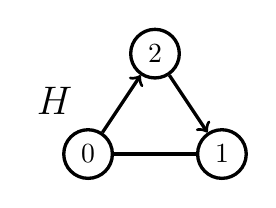
\begin{tikzpicture}[
    scale=0.85,
    minimum size=0.05cm,
    line width=1.2pt
]

    % ----------- Graf H ------------
    \node at (-1.5,1.8) {\Large \(H\)};

    \node[circle, draw=black] (v0) at (-1,1) {\(0\)};
    \node[circle, draw=black] (v1) at (1,1) {\(1\)};
    \node[circle, draw=black] (v2) at (0,2.5) {\(2\)};

    \draw      (v0) -- (v1);
    \draw[->]  (v0) -- (v2);
    \draw[->]  (v2) -- (v1);

\end{tikzpicture}

    \end{figure}
    \begin{figure}[H]
        \hspace{3em}
        \begin{tikzpicture}[
    scale=0.85,
    minimum size=0.05cm,
    line width=1.2pt
]

\begin{scope}[shift=({0,-3})]
    \node at (-1.5,1.8) {\Large \(R\)};

    \node[circle, draw=black] (v0) at (-1,1) {\(0\)};
    \node[circle, draw=black] (v1) at (1,1) {\(1\)};
    \node[circle, draw=black] (v2) at (0,2.5) {\(2\)};

    \draw[cfred] (v0) -- (v1);
    \draw[cfred] (v0) -- (v2);
    \draw[cfred, loop left] (v0) to node[left] {} (v0);
    \draw[cfred, loop right] (v1) to node[left] {} (v1);
    \draw[cfred, loop above] (v2) to node[left] {} (v2);
\end{scope}

\end{tikzpicture}

    \end{figure}
\end{columns}

\end{frame}

%---------------------------------------------------------

\begin{frame}{Przykład konstrukcji}

\begin{columns}
\column{0.55\textwidth}
    \vspace{2.5em}
    \begin{figure}[H]
        \centering
        \begin{tikzpicture}[
    scale=1,
    line width=1.2pt,
    minimum size=0.02cm
]

% Podświetlenie pp-def
\uncover<2>{
    \draw[rounded corners=5pt, draw=cfgrey!50, fill=cfgrey!50]
      (0.5,1.7) rectangle (1.6,3.5);
}

\uncover<3>{
    \draw[rounded corners=5pt, draw=cfgrey!50, fill=cfgrey!50]
      (-0.3,-0.8) rectangle (0.3,0.4);
}

\uncover<4>{
    \draw[rounded corners=5pt, draw=cfgrey!50, fill=cfgrey!50]
      (1.45,-0.8) rectangle (2.55,0.4);
}


    % Gadżet
    \node at (-1.6,0) {\large \(\DorD(u,v) \equiv\)};
    \node[circle, draw=black, fill=white, label=below:{\(0\)}]
            (x0) at (0,0) {};
    \node[circle, draw=black, fill=white] (x1) at (1,0) {};
    \node[circle, draw=black, fill=white, label=below:{\(\set{0,1}\)}]
            (x2) at (2,0) {};
    \node[circle, draw=black, fill=white] (x3) at (3,0) {};
    \node[circle, draw=black, fill=white, label=below:{\(1\)}]
            (x4) at (4,0) {};

    \node[circle, draw=black, fill=white] (x11) at (1,1) {};
    \node[circle, draw=black, fill=white] (x12) at (1,2) {};
    \node[circle, draw=black, fill=cfblue!50] (u) at (1,3) {\(u\)};

    \node[circle, draw=black, fill=white] (x31) at (3,1) {};
    \node[circle, draw=black, fill=white] (x32) at (3,2) {};
    \node[circle, draw=black, fill=cfblue!50] (v) at (3,3) {\(v\)};

    \draw[->] (x0) -- (x1);
    \draw[->] (x1) -- (x2);
    \draw[->] (x2) -- (x3);
    \draw[->] (x3) -- (x4);

    \draw[draw=cfred, line width=1.5]
      (u) -- node[midway, right] {\(R\)} (x12);
    \draw[->] (x12) -- (x11);
    \draw[->] (x11) -- (x1);

    \draw[draw=cfred, line width=1.5]
      (v) -- node[midway, right] {\(R\)} (x32);
    \draw[->] (x32) -- (x31);
    \draw[->] (x31) -- (x3);

\end{tikzpicture}

    \end{figure}

\column{0.45\textwidth}
    \vspace{1em}
    \begin{figure}[H]
        \hspace{3em}
        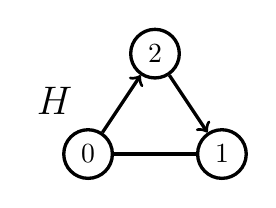
\begin{tikzpicture}[
    scale=0.85,
    minimum size=0.05cm,
    line width=1.2pt
]

    % ----------- Graf H ------------
    \node at (-1.5,1.8) {\Large \(H\)};

    \node[circle, draw=black] (v0) at (-1,1) {\(0\)};
    \node[circle, draw=black] (v1) at (1,1) {\(1\)};
    \node[circle, draw=black] (v2) at (0,2.5) {\(2\)};

    \draw      (v0) -- (v1);
    \draw[->]  (v0) -- (v2);
    \draw[->]  (v2) -- (v1);

\end{tikzpicture}

    \end{figure}
    \begin{figure}[H]
        \centering
        \begin{tikzpicture}[
    scale=1,
    line width=1.2pt
]

\uncover<2>{
    % Podświetlenie
    \draw[rounded corners=5pt, draw=cfgrey!50, fill=cfgrey!50]
      (-3.8,-0.7) rectangle (1.5,2);
      
        \node at (-2.4,0) {\large \(R(u,v) \equiv \)};

        \node[circle, draw=black, fill=white, label=below:{\(u\)}] (x0) at (-0.85,0) {};
        \node[circle, draw=black, fill=white] (x1) at (-0.4,0.7) {};
        \node[circle, draw=black, fill=white] (x2) at (0.05,1.4) {};
        \node[circle, draw=black, fill=white] (x3) at (0.5,0.7) {};
        \node[circle, draw=black, fill=white, label=below:{\(v\)}] (x4) at (0.95,0) {};

        \draw[->] (x0) -- (x1);
        \draw[->] (x1) -- (x2);
        \draw[->] (x3) -- (x2);
        \draw[->] (x4) -- (x3);
}

\uncover<3>{
    % Podświetlenie
    \draw[rounded corners=5pt, draw=cfgrey!50, fill=cfgrey!50]
      (-3.9,-0.7) rectangle (1.5,1.6);

    \node at (-2.4,0) {\large \((u = 0) \equiv \exists_{v, w}\)};
    \node[circle, draw=black, fill=white] (v0) at (-0.75,0) {\(u\)};
    \node[circle, draw=black, fill=white] (v1) at (0.75,0) {\(v\)};
    \node[circle, draw=black, fill=white] (v2) at (0,1) {\(w\)};

    \draw[<->] (v0) -- (v1);
    \draw[->]  (v0) -- (v2);
    \draw[->]  (v2) -- (v1);
}

\uncover<4>{
    % Podświetlenie
    \draw[rounded corners=5pt, draw=cfgrey!50, fill=cfgrey!50]
      (-4.25,-0.7) rectangle (1.5,0.9);

    \node at (-2.6,0) {\large \((u \in \set{0,1}) \equiv \exists_{v}\)};
    \node[circle, draw=black, fill=white] (v0) at (-0.75,0) {\(u\)};
    \node[circle, draw=black, fill=white] (v1) at (0.75,0) {\(v\)};

    \draw[<->] (v0) -- (v1);
}

\end{tikzpicture}

    \end{figure}
\end{columns}

\end{frame}

%---------------------------------------------------------

\begin{frame}{Przykład konstrukcji}

    Korzystając z relacji \(\DorD(u,v)\), definiujemy:
    \[ \textcolor{cfblue}{\eqoreq(a,b,c,d)} \equiv (a=b \lor c=d) \]

    \pause
    To wystarcza, żeby wyrazić problem NAE-SAT, który jest NP-zupełny.
    \begin{align*} 
        \textcolor{cfred}{\text{NAE-SAT}(u,v,w)} & \iff \neg\:(u = v = w) \\
        & \iff u \neq v \lor v \neq w \\
        & \iff \exists_{v'} \ v \neq v' \land (u=v' \lor v'=w) \\
        & \iff \exists_{v'} \ v \neq v' \land \textcolor{cfblue}{\eqoreq(u, v', v', w)}
    \end{align*}

\end{frame}
 